\documentclass{article}
\usepackage[a4paper, total={6in, 8in}]{geometry}
\usepackage{changepage}
\usepackage{multirow}
\usepackage{tocloft}
\usepackage{tabularx}
\usepackage{graphicx}
\usepackage{array}
\usepackage{tabu}
\usepackage{longtable}
\usepackage{wrapfig}
\usepackage{verbatim}
\usepackage{xltabular}
\usepackage[usenames,dvipsnames,table]{xcolor}

%creazione dei colori custom
\definecolor{tableGreen}{RGB}{25, 175, 45}
\definecolor{tableYellow}{RGB}{255, 220, 0}
\definecolor{tableBlue}{RGB}{0 ,20, 210}
\definecolor{tableCyan}{RGB}{0 ,160, 156}
\definecolor{tableRed}{RGB}{220 ,15, 5}

%macro per andare a capo nelle tabelle
\newcommand{\n}{
   \tabularnewline\hline
}

\tolerance=1
\hyphenpenalty=10000

%robe per tabelle
\renewcommand{\arraystretch}{2.4}%padding sopra sotto
\setlength\tabcolsep{6pt}%padding bordo lat


%macro per generare le tabelle
\newcommand{\monkeytable}[2]{
\begin{center}
\begin{tabularx}{\textwidth}
#2
\n %necessaria per chiudere la tabella
\end{tabularx}
\end{center}
\label{tab:monkeytable}
}

%inizio documento vero e proprio
\title{Codemonkey}
\begin{document}

\begin{comment}
\begin{figure}[!ht]
   \centering
   
\includegraphics[width=0.5\linewidth]{images/icon}
   \begin{titlepage}
      \huge Codemonkey
   \end{titlepage}
   \label{fig:nome-etichetta}
\end{figure}
\end{comment}


\pagebreak
\tableofcontents
\pagebreak
\section {Abstract}

L'obiettivo è sviluppare una piattaforma web che espone programmatori a realtà lavorative che ne hanno bisogno.
Sia i programmatori che le aziende si registrano al sito, e sono interfacciati al servizio Codemonkey attraverso pannelli diversi.
Un programmatore registrato inserisce i propri contatti, una breve descrizione e un elenco degli strumenti software nei quali ha competenze.
Un'azienda registrata può cercare programmatori filtrandoli per gli strumenti software dei quali ha esigenza. Quando l'azienda sceglie un programmatore, a questo arriva una notifica e può decidere di accettare il lavoro.
A lavoro concluso, l'azienda valuta il programmatore con un sistema di quotazione.
Il profilo del programmatore è aggiornato con i suoi lavori recenti.
\pagebreak
\section {\Large Raccolta dei requisiti}
\begin{itemize}
\large
\item Gli utenti del servizio Codemonkey si registrano da una pagina e indicano se intendono registrarsi come Codmonkey o Clienti
\item La Codmonkey potrá accedere, modificare i suoi dati e accettare eventuali lavori dopo aver eseguito l'Autenticazione
\item Un Cliente potrá accedere, modificare i suoi dati e gestire le Collaborazioni dopo aver eseguito il l'Autenticazione
\item Gli Utenti possono sfogliare il sito. Solo i clienti possono mandare richieste di Lavoro alle Codmonkey
\item Le Codmonkey possono accettare o rifiutare i lavori
\item I clienti possono valutare la Codmonkey solo dopo aver terminato la collaborazione e la valutazione potrá ache opzionalmente contenere una recensione
\item Si potranno cercare Codmonkey utlizzando dei filti specifici
\end{itemize}

\pagebreak
\section {Vocabolario}

\begin{table}[ht]
\begin{tabularx}{\textwidth}{|X|X|X|}
\hline
Voce & Definizione & Sinonimo \\
\hline
Programmatore & Utente registrato che fornisce uno o piú servizi alle aziende  & \\
\hline
Azienda & Azienda o un semplice privato interessato a utilizzare uno o piú servizi offerti da un programmatore & \\
\hline
Credenziali  & Metodo di accesso al servizio, basato su username e password & \\
\hline
Account & Insieme di Credenziali e informazioni che identifica una Azienda/Programmatore & \\
\hline
Utente & \begin{tabular}{@{}l@{}}Utilizzatore del servizio \\(Sia Azienda che \\ Programmatore)\end{tabular} & \\
\hline
Username & \begin{tabular}{@{}l@{}} Stringa alfanumerica \\ che identifica il nome \\dell'utente che sta \\ tentando l'accesso \end{tabular} & Identificativo\\
\hline
Password & \begin{tabular}{@{}l@{}}Stringa alfanumerica\\ generata da un utente\\ del servizio\end{tabular} & \\
\hline
Autenticazione & \begin{tabular}{@{}l@{}}Meccanismo di accesso \\ con nome alla \\piattaforma\end{tabular} &  Log in\\
\hline
Registrazione & Funzione di iscrizione alla piattaforma & \\
\hline
\end{tabularx}
\end{table}
\pagebreak
\section {Tabelle dei Requisiti}

\newcounter{greenC}

\newcommand{\tableGreen}{%onde evitare caos il colore della tabella viene dichiarato qui
    \\
    \rowcolor{tableGreen!15}
    \hline
    \stepcounter{greenC}
    R\thegreenC F
}

\newcommand{\ntableGreen}{
    \\
    \rowcolor{tableGreen!5}
    \hline
    \stepcounter{greenC}
    R\thegreenC F
}

\monkeytable{3} {
{|>{\arraybackslash}m{1.5cm}|>{\centering\arraybackslash}X|}

\hline
\rowcolor{tableGreen!70}
\multicolumn{2}{|c|}{\textbf{Requisiti Funzionali}}
\n \rowcolor{tableGreen!50} \textbf{ID} & \textbf{Requisito}
\ntableGreen    & un utente qualsiasi può sfogliare il sito e vedere tutti i programmatori
\tableGreen     & il sito deve fornire la possibilità di inserire dei filtri per cercare programmatori con specifiche caratteristiche
\ntableGreen    & è presente una sezione nella quale un utente o una azienda possono autenticarsi
\tableGreen     & è presente una sezione nella quale un utente o una azienda possono registrarsi
\ntableGreen    & una azienda potrà contattare un programmatore solo previa autenicazione
\tableGreen     & un programmatore può accedere previa autenticazione alla pagina del suo profilo
\ntableGreen    & possono essere effettuate modifiche delle informazioni del programmatore dalla pagina principale
\tableGreen     & possono essere accettati i lavori e mandati i preventivi sempre da essa
\ntableGreen    & viene fornita la valutazione di ogni programmatore anche filtrata secondo specifici linguaggi
\tableGreen     & viene fornita la possibilità di vedere se un programmatore sta lavorando ad un progetto o meno
}
\newcounter{yellowC}

\newcommand{\Yellow}{%onde evitare caos il colore della tabella viene dichiarato qui
    \\
    \rowcolor{tableYellow!15}
    \hline
    \stepcounter{yellowC}
    R\theyellowC NF
}

\newcommand{\nYellow}{
    \\
    \rowcolor{tableYellow!5}
    \hline
    \stepcounter{yellowC}
    R\theyellowC NF
}
\monkeytable{3} {
{|>{\arraybackslash}m{1.5cm}|>{\arraybackslash}X|}

\hline
\rowcolor{tableYellow!70}
\multicolumn{2}{|c|}{\textbf{Requisiti Non Funzionali}}
\n \rowcolor{tableYellow!50} \textbf{ID} & \centering\textbf{Requisito} \endline
\rowcolor{tableYellow!15}
\hline
\stepcounter{yellowC}
R\theyellowC NF 
            & Il sito deve essere facile da navigare
\nYellow    & Deve essere tracciata l'attivitá dei vari amministratori
\Yellow     & Viene fornita la Valutazione Generale di ogni Codmonkey
\nYellow    & Viene fornita una Valutazione Filtrata del programmatore in base ai filtri impostati nella ricerca del Cliente
\Yellow     & Deve essere possibile vedere a qunti progetti la Codmonkey sta lavorando

}
\newcounter{reqDCounter}%counter

\newcommand{\nReqD}{
    \n
    \stepcounter{reqDCounter}
    R\thereqDCounter D
}

\begin{center}
    \rowcolors{2}{tableBlue!4}{tableBlue!8}%colori alternati
    \begin{tabularx}{\textwidth}
        {|c|X|}
        \hline\rowcolor{tableBlue!50}
        \multicolumn{2}{|c|}{\Large\textbf{Requisiti di Dominio}}
        \n \rowcolor{tableBlue!25} \large\textbf{ID}
               & \large\textbf{Requisito}
        \nReqD & Non é necessaria l'autenticazione per eseguire una rcerca di Codmonkey
        \nReqD & Gli amministratori del sistema devono essere creati prima dell'avvio del sistema e non se ne possono aggiungere durante l'esecuzione
        \nReqD & Non sará possibile regisrtarsi si come codmonkey che come Cliente
        \nReqD & Un Utente Registrato in qualsiasi momento puó richiedere l'eliminazione del suo Account
        \n
    \end{tabularx}
\end{center}
\pagebreak
%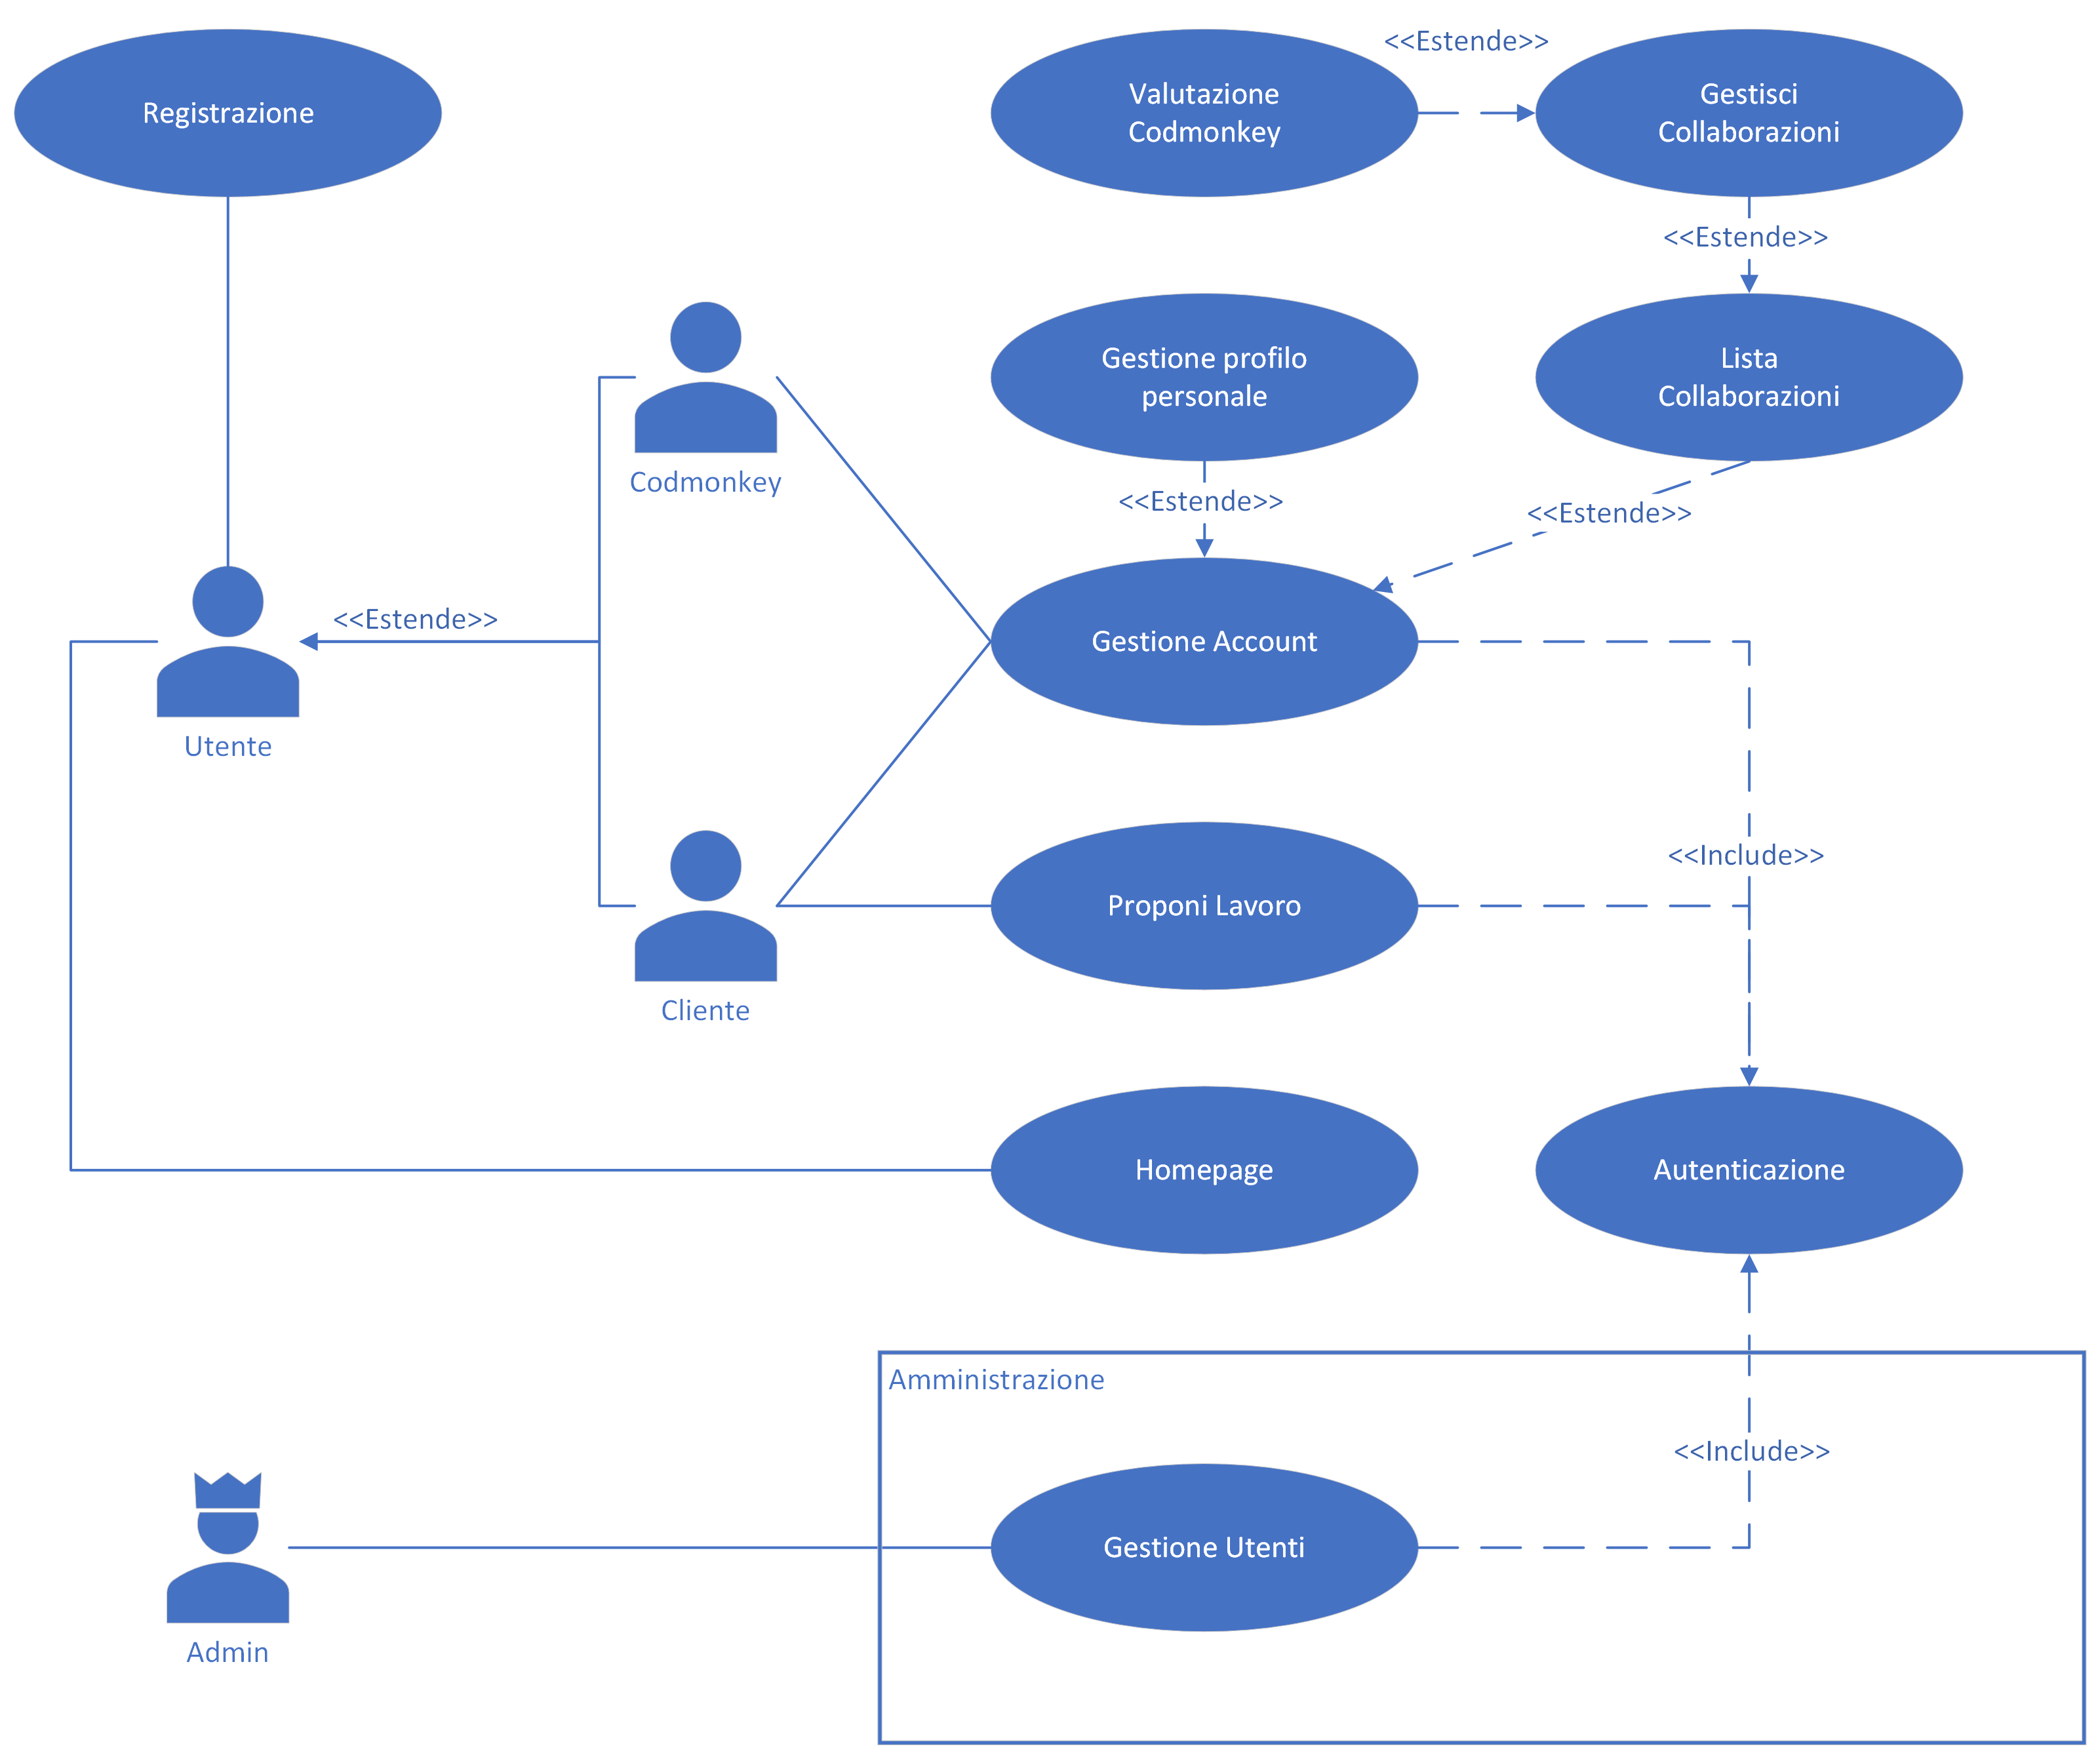
\includegraphics[width=\textwidth]{images/Codmonkey Casi D'uso.png}\label{fig:CasiUso}
\pagebreak
\section {Scenari}


\newcommand{\tableCyan}{%onde evitare caos il colore della tabella viene dichiarato qui
    \\
    \hline 
    \rowcolor{tableCyan!10}
    \cellcolor{tableCyan!22}
}

\newcommand{\ntableCyan}{
    \\
    \hline
    \rowcolor{tableCyan!5}
    \cellcolor{tableCyan!12}
}


\monkeytable{3} {
{|>{\arraybackslash }m{3cm}|>{\arraybackslash}X|}

\hline \rowcolor{tableCyan!37} \centering\textbf{Titolo} & \centering\textbf{...}\endline
\hline 
\rowcolor{tableCyan!10}
\cellcolor{tableCyan!22}

               Descrizione &test
\ntableCyan    Attori &
\tableCyan     Relazioni &
\ntableCyan    Precondizioni &
\tableCyan     Postcondizioni &
\ntableCyan    Scenario Principale &
\tableCyan     Scenari Alternativi &
\ntableCyan    Requisiti NF &
\tableCyan     Punti Aperti &
}










    % NO    % NO    % NO    % NO    % NO
% NO    % NO    % NO    % NO    % NO

%Si usa per il copia e incolla
%Non  riempitela scimmieeeee                                       monke

\monkeytable{3} {
{|>{\arraybackslash }m{3cm}|>{\arraybackslash}X|}

\hline \rowcolor{tableCyan!37} \centering\textbf{Titolo} & \centering\textbf{...}\endline
\hline 
\rowcolor{tableCyan!10}
\cellcolor{tableCyan!22}

               Descrizione &test
\ntableCyan    Attori &
\tableCyan     Relazioni &
\ntableCyan    Precondizioni &
\tableCyan     Postcondizioni &
\ntableCyan    Scenario Principale &
\tableCyan     Scenari Alternativi &
\ntableCyan    Requisiti NF &
\tableCyan     Punti Aperti &
}

    % NO    % NO    % NO    % NO    % NO
% NO    % NO    % NO    % NO    % NO
                                                                                                                                         %un simpatico easter egg

\pagebreak
\section{Analisi del rischio}
    
\renewcommand{\arraystretch}{2}%padding sopra sotto
\setlength\tabcolsep{5pt}%padding bordo lat
\rowcolors{2}{tableRed!15}{tableRed!6}%colori alternati
\begin{center}
\begin{adjustwidth}{-1.8cm}{0cm} 
\resizebox{1.3\textwidth}{!}{%tabella piú larga
\begin{tabular}{|m{4cm}|m{6cm}|m{5cm}|}

\hline  \rowcolor{tableRed!70}  \multicolumn{3}{|c|}{\textbf{Valutazione dei beni}}
\n      \rowcolor{tableRed!50}  \textbf{Bene} &  \textbf{Valore} &   \textbf{Esposizione}

\n      Credenziali di accesso Codemonkey&Alto:\newline
        Possibilità di modificare le informazioni relative alle Codemonkey.\newline
        Possibilità di rifiutare lavori per conto delle Codemonkey&
        Alta:\newline
        Possibilie perdita economica per la Codemonkey\newline
        Danno di immagine

\n      Credenziali di accesso Clienti&
        Alto:\newline
        Possibilità di proporre lavori fasulli\newline
        Possono essere scritte recensioni false&
        Alta:\newline
        Costi di ripristino\newline
        Possibili spese di rimborso per lavori fasulli già iniziati\newline
        Danno di immmagine

\n      Credenziali di accesso Amministratori&
        Molto Alto\newline
        Completa gestione di tutti gli Utenti registrati\newline
        Possibilità di vedere lavori non ancora terminati&
        Molto Alta:\newline
        Costi di ripristino di sistema\newline
        Possibile danno di immagine nel caso la notizia diventi di pubblico dominio

\n      DB Utenti Registrati&
        Alto:\newline
        Accesso a tutti i dati degli Utenti registrati&
        lo mettiamo?
                
\n
\end{tabular}
}
\label{tab:monkeytable:monkerisk:valutaBanane}
\end{adjustwidth}

\begin{adjustwidth}{-2.6cm}{0cm} 
\centering
\resizebox{1.4\textwidth}{!}{
\begin{tabular}{|m{3.25cm}|m{4cm}|m{4.75cm}|m{4cm}|}
 
\hline  \rowcolor{tableRed!70}  \multicolumn{4}{|c|}{\textbf{Minacce e Controlli}}
\n      \rowcolor{tableRed!50}  \textbf{Minaccia} &  \textbf{Probabilità} &   \textbf{Controllo} & \textbf{Fattibilità} 

\n      Furto identità Amministratore &
        Molto Bassa\newline
        Username e password stabiliti dall'Amministratore insieme a un sistema per autenticazione a 2 fattori&
        Numero di tentativi disponibili limitato nel tempo\newline
        Autenticazione a 2 fattori che rende valida la sessione corrente\newline
        Log di ogni tentativo di accesso&
        Costo di implementazione Medio-Basso
\n      Furto identità cliente o Codemonkey&
        Media o Bassa\newline
        Username e password scelti in fase di registrazione&
        Numero di tentativi disponibili limitato nel tempo\newline
        Possibilità per un utente registrato di attivare l'autenticazione a 2 fattori\newline
        Possibilità di recuperare l'accouynt tramite mail&
        Costo di implementazione Medio-Basso\newline
\n      Intercettazione delle comunicazioni&
        Media\newline
        Il servizio è realizzato in rete&
        Utilizzo di un sistema crittografico per la cifratura delle comunicazioni&
        Costo di implementazione Basso\newline
\n      Deny of Service&
        Bassa\newline
        Bassa probabilità di un attacco dos&
        Numero di operazioni di rete possibili limitato nel tempo&
        Basso Costo\newline
        Gestione delle richieste e della rete delegata agli Amministratori
\n

\end{tabular}
\label{tab:monkeytable:monkerisk:monkeMinacciataMaMonkeControlla}
}
\end{adjustwidth}

\newpage
\begin{tabular}{|m{4cm}|m{7cm}|}
\hline \rowcolor{tableRed!70}  \multicolumn{2}{|c|}{\textbf{Tecnologia e Vulnerabilità}}
\n \rowcolor{tableRed!50}  \textbf{Tecnologia} &  \textbf{Vulnerabilità}  
\n  Autenticazione & 
        Utente registrato rivela username e password volontariamente o per errore e non ha attivato l'autenticazione a due fattori
\n      Architettura Client/Server &
        Attacco Deny of Service\newline
        Intercettazione delle comunicazioni:\newline
        Man in the middle, Sniffing
\n
\end{tabular}
\label{tab:monkeytable:monkerisk:monkeVulnerabile}

\end{center}


\pagebreak
%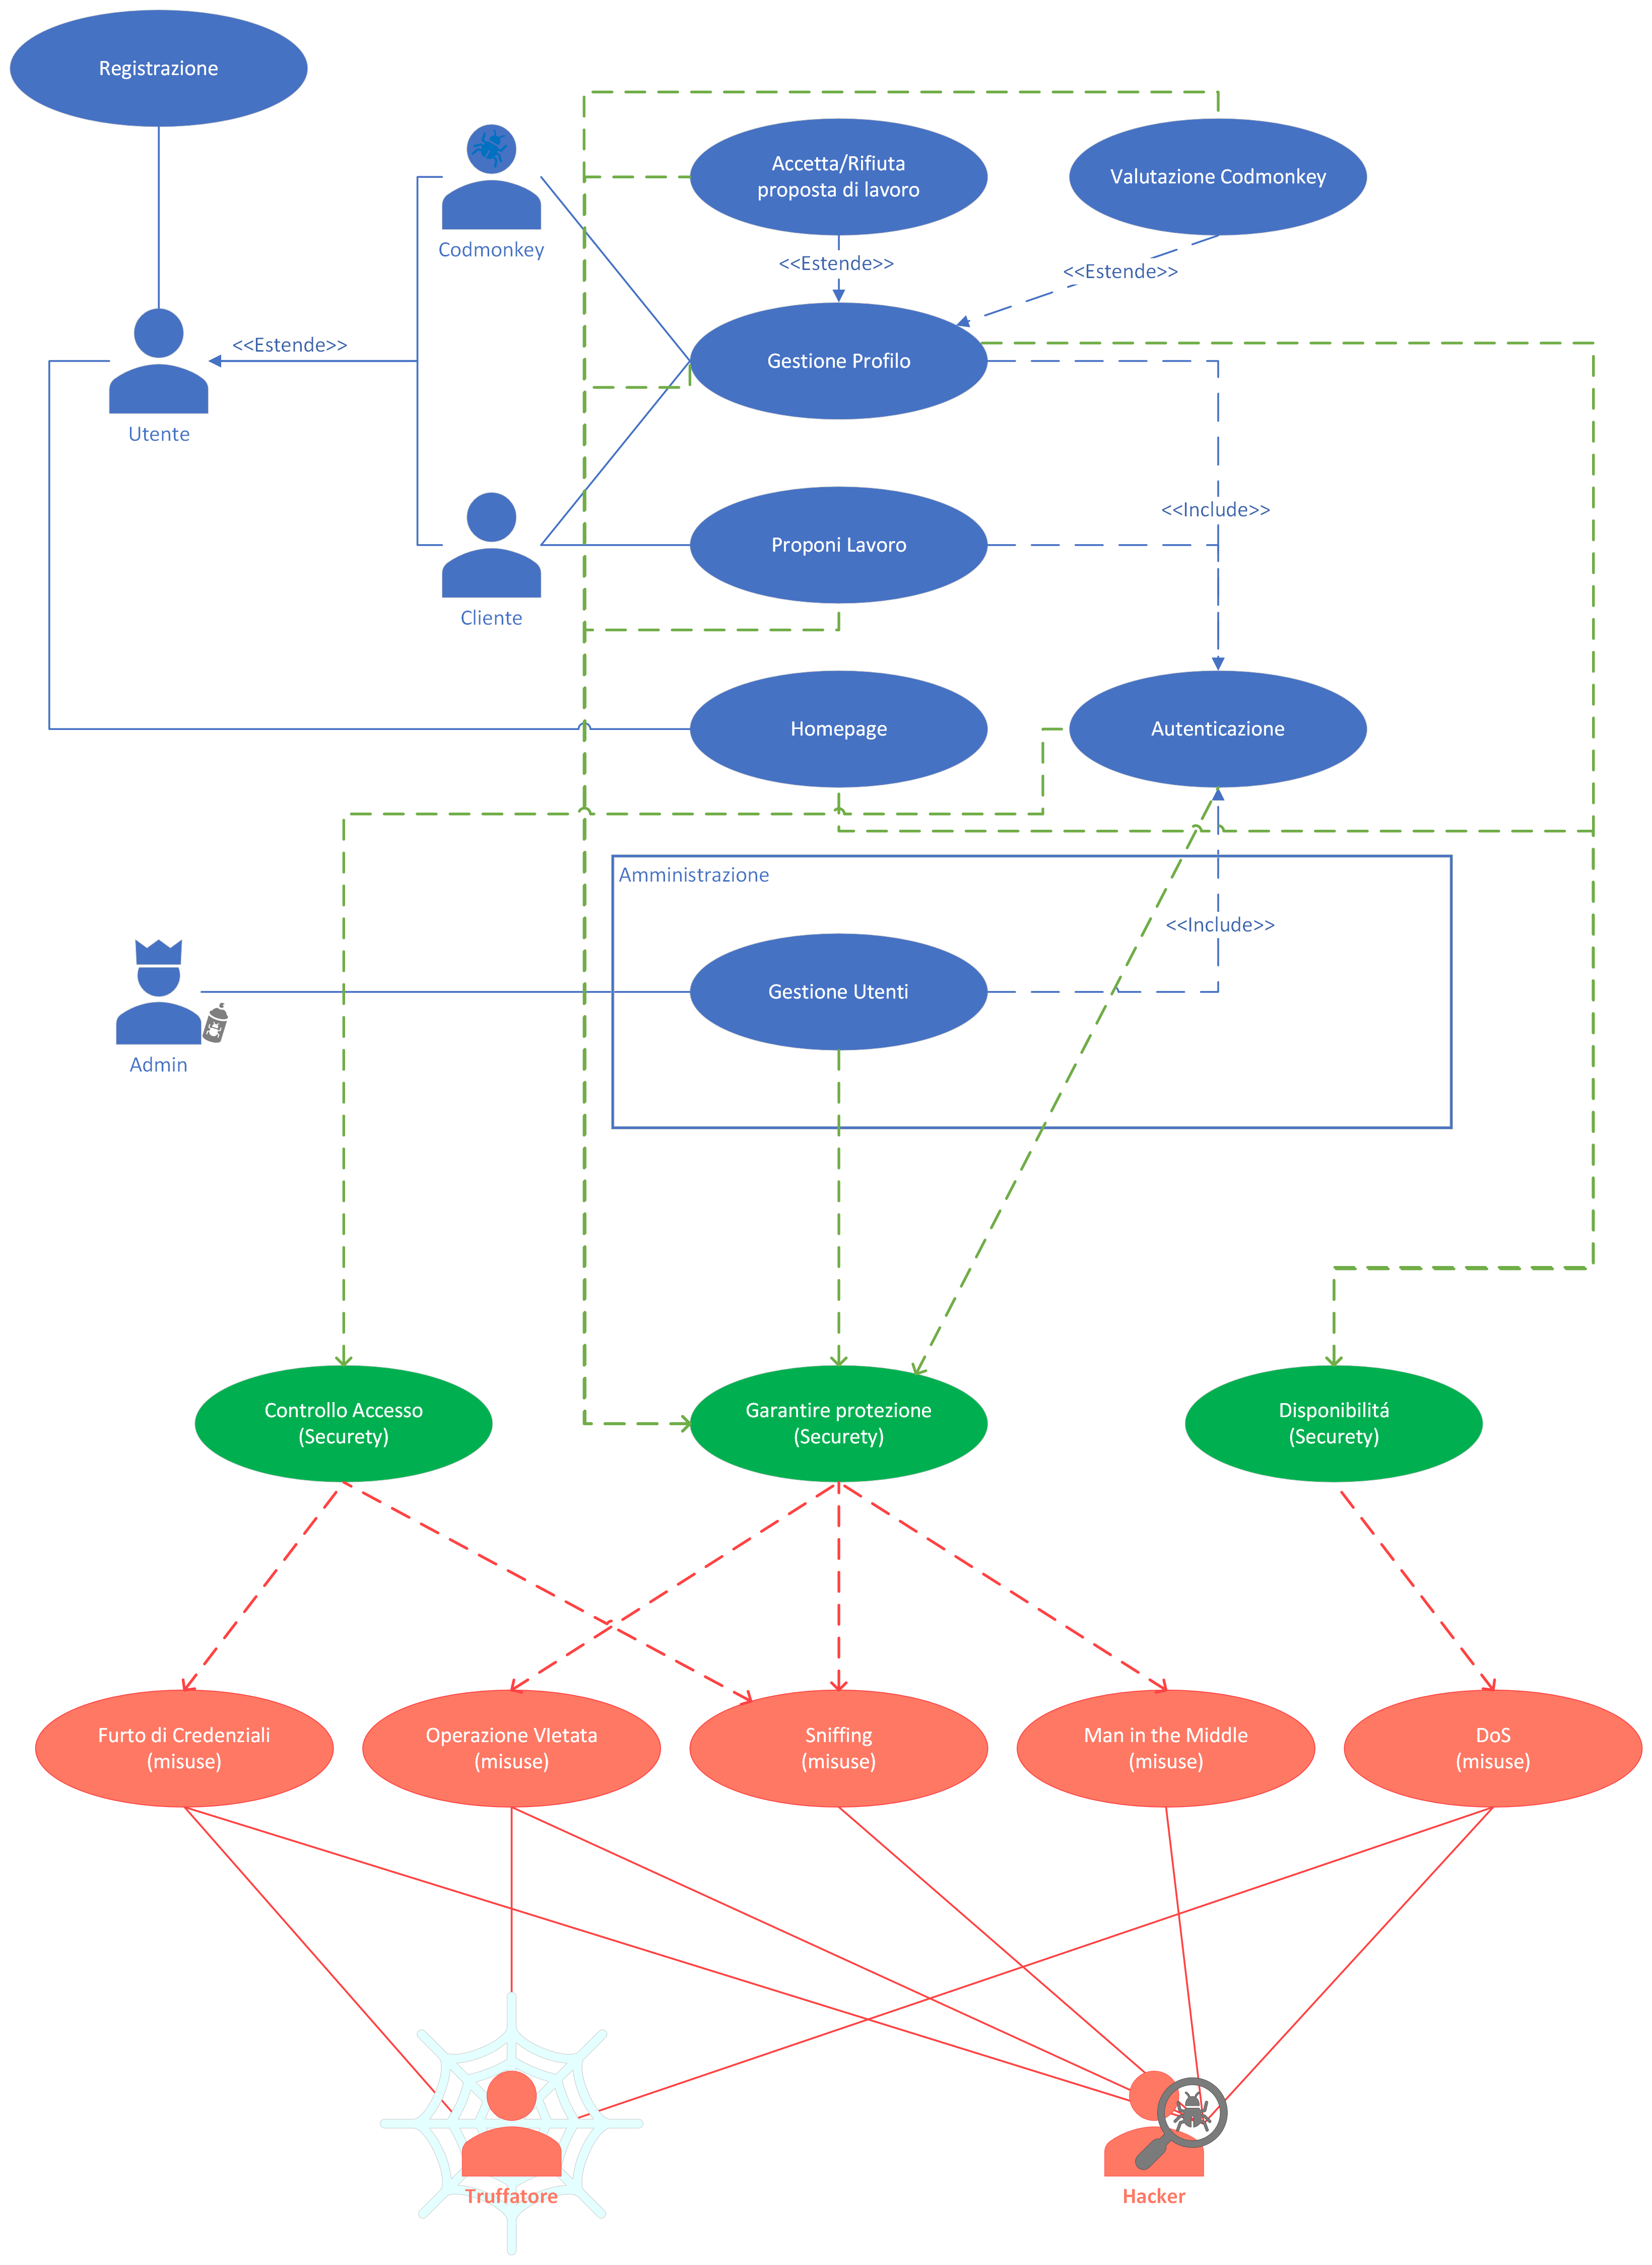
\includegraphics[width=\textwidth]{images/Codmonkey Security Use Case e Misuse Case.png}\label{fig:SecuretyUseCaseAndMissuseCase}
\section{Use and Misuse Case scenari}

\begin{center}%%%%%%%%%%%%%%%
    



\renewcommand{\arraystretch}{2}%padding sopra sotto
\setlength\tabcolsep{5pt}%padding bordo lat
\rowcolors{2}{orange!20}{orange!5}%colori alternati
\begin{adjustwidth}{-1.8cm}{0cm}
    \resizebox{1.3\textwidth}{!}{%tabella piú larga
    \begin{tabular}
    {|m{4.5cm}|m{4cm}|m{4cm}|}%Opzioni per formato tabella
    \hline
    \rowcolor{orange!50}%settare il colore della riga 
    \textbf{Titolo} &\multicolumn{2}{|c|}{\textbf{Disponibilitá}} %voci della prima colonna
    \n  Descrizione&\multicolumn{2}{|l|}{tette}
    \n  Misuse Case&\multicolumn{2}{|l|}{}
    \n  Precondizioni&\multicolumn{2}{|l|}{}
    \n  Postcondizioni&\multicolumn{2}{|l|}{}
    \n  Scenario Principale&&
    \n  Scenario di attacco avvenuto con successo&&
    \n
    \end{tabular}
    }
    \label{tab:monkeytable:riskmonke:lianaSicuraOMarcia}
\end{adjustwidth}



%%%%%%%%%%%%%%%%%%%%%%%%%%%%%%%%%%%%%%



\begin{adjustwidth}{-1.8cm}{0cm}
    \resizebox{1.3\textwidth}{!}{%tabella piú larga
    \begin{tabular}
    {|m{4.5cm}|m{4cm}|m{4cm}|}%Opzioni per formato tabella
    \hline
    \rowcolor{orange!50}%settare il colore della riga 
    \textbf{Titolo} &\multicolumn{2}{|c|}{\textbf{Gatantire protezione}} %voci della prima colonna
    \n  Descrizione&\multicolumn{2}{|l|}{culo}
    \n  Misuse Case&\multicolumn{2}{|l|}{}
    \n  Precondizioni&\multicolumn{2}{|l|}{}
    \n  Postcondizioni&\multicolumn{2}{|l|}{}
    \n  Scenario Principale&&
    \n  Scenario di attacco avvenuto con successo&&
    \n
    \end{tabular}
    }
    \label{tab:monkeytable:riskmonke:lianaSicuraOMarcia}
\end{adjustwidth}



%%%%%%%%%%%%%%%%%%%%%%%%%%%%%%%%%%%%%%%%%%%%%%%%%



\begin{adjustwidth}{-1.8cm}{0cm}
    \resizebox{1.3\textwidth}{!}{%tabella piú larga
    \begin{tabular}
    {|m{4.5cm}|m{4cm}|m{4cm}|}%Opzioni per formato tabella
    \hline
    \rowcolor{orange!50}%settare il colore della riga 
    \textbf{Titolo} &\multicolumn{2}{|c|}{\textbf{Controllo accesso}} %voci della prima colonna
    \n  Descrizione&\multicolumn{2}{|l|}{bocca}
    \n  Misuse Case&\multicolumn{2}{|l|}{}
    \n  Precondizioni&\multicolumn{2}{|l|}{}
    \n  Postcondizioni&\multicolumn{2}{|l|}{}
    \n  Scenario Principale&&
    \n  Scenario di attacco avvenuto con successo&&
    \n
    \end{tabular}
    }
    \label{tab:monkeytable:riskmonke:lianaSicuraOMarcia}
\end{adjustwidth}



\end{center}%%%%%%%%%%%%%%%%%%%%%%%




\pagebreak

\begin{center}
    \rowcolors{2}{tableGreen!5}{tableGreen!10} %colori alternati
    \begin{tabularx}{\textwidth}
        {|c|X|}
        \hline\rowcolor{tableGreen!60}
        \multicolumn{2}{|c|}{\Large\textbf{Requisiti Funzionali Aggiornati}}
        \n \rowcolor{tableGreen!35} \large\textbf{ID}
               & \large\textbf{Requisito}
        \nReqF & Creazone di un file di Log per tenere traccia delle operazioni
        \nReqF & L'Amministratore avrá la possibilitá di vedere tutte le operazioni salvate all'interno del file di Log e porá anche scaricare il file
        \n
    \end{tabularx}


    \phantom{M}%%%%%%%%%%%%%%%%%%%%%%%%%%%%%%%%%%


    \rowcolors{2}{tableYellow!5}{tableYellow!10} %colori alternati
    \begin{tabularx}{\textwidth}
        {|c|X|}
        \hline\rowcolor{tableYellow!60}
        \multicolumn{2}{|c|}{\Large\textbf{Requisiti Non Funzionali Aggiornati}}
        \n \rowcolor{tableYellow!35} \large\textbf{ID}
                & \large\textbf{Requisito}
        \nReqNF & Il sistema deve ripristinarsi velocemene in caso di attacco
        \nReqNF & Verrá eseguito un backup periodico dello stato del sistema
        \n
    \end{tabularx}


    \phantom{M}%%%%%%%%%%%%%%%%%%%%%%%%%%%%%%%%%%


    \rowcolors{2}{orange!6}{orange!10} %colori alternati
    \begin{tabularx}{\textwidth}
        {|c|>{\raggedright}X|l|}

        \hline \rowcolor{orange!60}
        \multicolumn{3}{|c|}{\Large\textbf{Vocabolario Aggiornato}}

        \n \rowcolor{orange!40}
        \Large\textbf{Voce} & \Large\centering\textbf{Definizione}                                  & \Large\textbf{Sinonimo} %voci della prima colonna
        \n Log              & File contenenete tutte le operazioni eseguite all'interno del sistema & File di Log
        \n
    \end{tabularx}
\end{center}


\section{Casi d'uso aggiornati}


\begin{tabularx}{\textwidth}{|c|X|}
    \hline \rowcolor{tableCyan!37} \large\centering\textbf{Titolo} & \large\centering\textbf{Visualizza Log}
    \tableCyan      Descrizione                                    & Pagina di monitoraggio dei Log
    \ntableCyan     Attori                                         & Amministratore
    \tableCyan      Relazioni                                      & Autenticazione
    \ntableCyan     Precondizioni                                  &
    \tableCyan      Postcondizioni                                 &
    \ntableCyan     Scenario Principale                            &
    \begin{enumerate}
        \item L'amministratore si autentica
        \item L'amministratore accede alla sezione dei Log
        \item L'amministraatore del gruppo può visualizzare i Log di sistema
        \item L'amministratore puó scaricare il file di Log
    \end{enumerate}
    \tableCyan      Scenari Alternativi                            &
    \ntableCyan     Requisiti NF                                   &
    \tableCyan      Punti Aperti                                   &
    \n
\end{tabularx}

\pagebreak
\section{Analisi delle funzionalitá}

\begin{center}

    \rowcolors{2}{tableGreen!6}{tableGreen!12}%colori alternati

    \begin{longtable}
        {|>{\centering}m{3.5cm}|m{4.5cm}|>{\centering}m{2.5cm}|>{\raggedright}m{2.5cm}|}
        \hline  \rowcolor{tableGreen!70}
        \multicolumn{4}{|c|}{\Large\textbf{Tabella delle Funzionalitá}}
        \n      \rowcolor{tableGreen!50}
        \large \textbf{Funzionalitá}                                            & \centering\large\textbf{Tipo}                                               & \large\textbf{Complessitá} & \centering\large\textbf{Reqisiti}
        \n
        \endhead                    Registrazione                               & Memorizzazione dati                                                         & Semplice                   & R1F
        \n                          Autenticazione                              & Interazione con l'esterno\newline Gestione dati                             & Semplice                   & R2F
        \n                          Homepage                                    & Interazione con l'estreno                                                   & Complessa                  & R3F, R6F, R11F, R12F
        \n                          Proponi lavoro                              & Interazione con l'esterno\newline Memorizzazione dati\newline Gestione dati & Semplice                   & R8F, R9F, R12F
        \n \rowcolor{tableGreen!35} Gestione Account                            & Interazione con l'esterno\newline Memorizzazione dati\newline Gestione dati & Complessa                  &
        \n \rowcolor{tableGreen!20} Modifica contatti                           & Interazione con l'esterno\newline Memorizzazione dati\newline Gestione dati & Semplice                   & R4F
        \n \rowcolor{tableGreen!20} Cambia dati personali                       & Interazione con l'esterno\newline Memorizzazione dati\newline Gestione dati & Complessa                  & R4F
        \n \rowcolor{tableGreen!20} Cambia password                             & Interazione con l'esterno\newline Memorizzazione dati\newline Gestione dati & Semplice                   & R4F
        \n \rowcolor{tableGreen!20} Impostazione autenticazione a 2 fattori     & Interazione con l'esterno\newline Gestione dati                             & Semplice                   & R4F
        \n \rowcolor{tableGreen!20} Elimina account                             & Interazione con l'esterno\newline Memorizzazione dati\newline Gestione dati & Semplice                   & R4F
        \n \newpage                  Lista collaborazioni                       & Interazione con l'esterno                                                   & Semplice                   & R4F
        \n                          Termina Collaborazione e Valuta Codmonkey   & Interazione con l'esterno\newline Memorizzazione dati\newline Gestione dati & Semplice                   & R10F
        \n \rowcolor{tableGreen!35} Accetta/Rifiuta /Termina proposta di lavoro & Interazione con l'esterno\newline Memorizzazione dati\newline Gestione dati & Semplice                   & R10F
        \n \rowcolor{tableGreen!20} Accetta Lavoro                              & Interazione con l'esterno\newline Memorizzazione dati\newline Gestione dati & Semplice                   & R10F
        \n \rowcolor{tableGreen!20} Rifiuta Lavoro                              & Interazione con l'esterno\newline Memorizzazione dati\newline Gestione dati & Semplice                   & R10F
        \n \rowcolor{tableGreen!20} Termina Lavoro                              & Interazione con l'esterno\newline Memorizzazione dati\newline Gestione dati & Semplice                   & R10F
        \n \newpage
        \rowcolor{tableGreen!35}    Gestione Utenti                             & Interazione con l'esterno\newline Gestione dati                             & Complessa                  & R7F
        \n \rowcolor{tableGreen!20} Limita Utente Registrato                    & Interazione con l'esterno\newline Gestione dati                             & Semplice                   & R7F
        \n \rowcolor{tableGreen!20} Sospendi Utente Registrato                  & Interazione con l'esterno\newline Gestione dati                             & Semplice                   & R7F
        \n \rowcolor{tableGreen!20} Blocca Utente Registrato                    & Interazione con l'esterno\newline Gestione dati                             & Semplice                   & R7F
        \n \rowcolor{tableGreen!20} Elimina Utente Registrato                   & Interazione con l'esterno\newline Gestione dati                             & Semplice                   & R7F
        \n \rowcolor{tableGreen!20} Gestisci filtri di ricerca                  & Interazione con l'esterno\newline Gestione dati
        \n                          Segnala un problema                         & Interazione con l'esternoGestione dati                                      & Semplice                   & R10F
        \n                          Visualizza log                              & Interazione con l'esterno                                                   & Semplice                   & R13F
        \n
    \end{longtable}
    \label{tab:monkeytable:problema:analisiFunzionalita}
\end{center}

%\n \pagebreak %da togliere il commento per andare a capo









\begin{comment}
...
\end{comment}
\pagebreak
\section{Tabella di Informazione/Flusso}

\begin{center}

    %%%%%%%%%%%%
    %% Utils  %%
    %%%%%%%%%%%%

    \newcommand{\headerFlusso}{% Header delle tabelle da utilizzare solo dopo il titolo
        \n
        \rowcolor{tableGreen!50}
        \large \textbf{Informazione} & \large\textbf{Tipo} & \large\textbf{Livello protezione /privacy} & \large\textbf{Input /Output} & \centering\large\textbf{Vincoli}
    }

    \rowcolors{2}{tableGreen!6}{tableGreen!12} %colori alternati

    %%%%%%%%%%%%%%%%%%%%%%%%%%%%%%%%%%%%%


    %%%%%%%%%%%%%
    %% Tables  %%
    %%%%%%%%%%%%%


    \begin{tabularx}{\textwidth}
        {|>{\centering}m{2.7cm}|>{\centering}m{1.65cm}|>{\centering}m{2.6cm}|>{\centering}m{2.2cm}|>\raggedright X|}
        \hline
        \rowcolor{tableGreen!70}
        \multicolumn{5}{|c|}{\Large\textbf{Registrazione}}
        \headerFlusso
        \n  Username & Complesso & Medio      & Input & Lunghezza di massimo 42 caratteri\newline Non saranno accettati caratteri speciali
        \n  Password & Semplice  & Molto Alto & Input & Almeno 8 caratteri massimo 42
        \n
    \end{tabularx}
    \label{tab:monkeytable:problema:tabFlusso:registrazione}



    \phantom{M} %%%%%%%%%%%%%%%%%%%%%%%%%%%%%



    \begin{tabularx}{\textwidth}
        {|>{\centering}m{2.7cm}|>{\centering}m{1.65cm}|>{\centering}m{2.6cm}|>{\centering}m{2.2cm}|>\raggedright X|}
        \hline
        \rowcolor{tableGreen!70}
        \multicolumn{5}{|c|}{\Large\textbf{Autenticazione}}
        \headerFlusso
        \n  Username & Semplice & Medio      & Input & Lunghezza di massimo 42 caratteri\newline Non saranno accettati caratteri speciali
        \n  Password & Semplice & Molto Alto & Input & Almeno 8 caratteri, massimo 42
        \n
    \end{tabularx}
    \label{tab:monkeytable:problema:tabFlusso:autenticazione}


    \phantom{M} %%%%%%%%%%%%%%%%%%%%%%%%%%%%%



    \begin{tabularx}{\textwidth}
        {|>{\centering}m{2.7cm}|>{\centering}m{1.65cm}|>{\centering}m{2.6cm}|>{\centering}m{2.2cm}|>\raggedright X|}
        \hline
        \rowcolor{tableGreen!70}
        \multicolumn{5}{|c|}{\Large\textbf{Homepage}}
        \headerFlusso
        \n               Profilo pubblico Codmonkey & Complesso & Pubblico & Output &
        \tabularnewline \textbf{Composto da:}       &           &          &        &
        \tabularnewline Nome Codmonkey              & Semplice  & Pubblico & Output & Massimo 32 caratteri
        \tabularnewline Filtri di ricerca           & Semplice  & Pubblico & Output & Filtri di massimo 32 caratteri, massimo 32 filtri per Codmonkey
        \tabularnewline Descrizione                 & Semplice  & Pubblico & Output & Descrizione della Codmonkey e di ció che sa fare di massimo 1024 caratteri
        \tabularnewline Valutazioni Codmonkey       & Semplice  & Pubblico & Output & Le Valutazioni generali e filtrate delle codmonkey andranno da un minimo di 1 a un massimo di 10
        \tabularnewline Immagine Profilo Codmonkey  & Semplice  & Pubblico & Output & Immagine di dimensioni limitate a 512x512 pixel
        \n              Casella di ricerca          & Semplice  & Pubblico & Input  & Sezione nella quale immettere la chiave di ricerca per trovare delle Codmonkey adatte alle proprie esigenze
        \n
    \end{tabularx}
    \label{tab:monkeytable:problema:tabFlusso:homepage}


    \phantom{M} %%%%%%%%%%%%%%%%%%%%%%%%%%%%%


    \begin{tabularx}{\textwidth}
        {|>{\centering}m{2.7cm}|>{\centering}m{1.65cm}|>{\centering}m{2.6cm}|>{\centering}m{2.2cm}|>\raggedright X|}
        \hline
        \rowcolor{tableGreen!70}
        \multicolumn{5}{|c|}{\Large\textbf{Proponi Lavoro}}
        \headerFlusso
        \n              Descrizione della proposta di Lavoro & Semplice & Basso & Input & Casella testuale nella quale sará descritto il lavoro richiesto dal Cliente\newline Almeno 255 carattri, massimo 2047 caratteri
        \n              Invia Proposta di Lavoro             & Sempice  & Basso & Input &
        \n
    \end{tabularx}
    \label{tab:monkeytable:problema:tabFlusso:proponiLavoro}


    \phantom{M} %%%%%%%%%%%%%%%%%%%%%%%%%%%%%


    \begin{tabularx}{\textwidth}
        {|>{\centering}m{2.7cm}|>{\centering}m{1.65cm}|>{\centering}m{2.6cm}|>{\centering}m{2.2cm}|>\raggedright X|}
        \hline
        \rowcolor{tableGreen!70}
        \multicolumn{5}{|c|}{\Large\textbf{}}
        \headerFlusso
        \n              &  &  &  &
        \tabularnewline &  &  &  &
        \n
    \end{tabularx}
    \label{tab:monkeytable:problema:tabFlusso:}


    \phantom{M} %%%%%%%%%%%%%%%%%%%%%%%%%%%%%




\end{center}







\begin{comment}

\tabularnewline \textbf{Composto da:} &  &  &  &

\tabularnewline  &  &  &  &

\n  &  &  &  &




\begin{tabularx}{\textwidth}
    {|>{\centering}m{2.7cm}|>{\centering}m{1.65cm}|>{\centering}m{2.6cm}|>{\centering}m{2.2cm}|>\raggedright X|}
    \hline
    \rowcolor{tableGreen!70}
    \multicolumn{5}{|c|}{\Large\textbf{Accetta/Rifiuta/Termina proposta di lavoro}}
    \headerFlusso
    \n Proposta di lavoro                              & Complesso & Medio & Output & Massimo 5 proposte di lavoro per Codmonkey
    \tabularnewline     \textbf{Composto da:}          &           &       &        &
    \tabularnewline     Nome Cliente                   & Semplice  & Basso & Output & Nome del Cliente di massimo 32 caratteri
    \tabularnewline     Descrizione proposta di lavoro & Semplice  & Medio & Input  & Massimo 255 caratteri
    \n                  Lavoro                         & Complesso & Medio & Output &
    \tabularnewline     \textbf{Composto da:}          &           &       &        &
    \tabularnewline     Nome Cliente                   & Semplice  & Basso & Output & Massio 32 caratteri
    \tabularnewline     Descrizione proposta di lavoro & Semplice  & Medio & Input  & Massimo 255 caratteri
    \n                  Interrompi lavoro              & Semplice  & Medio & Input  & Massimo 255 caratteri
    \n                  Segnala lavoro                 & Semplice  & Alto  & Input  & Massimo 255 caratteri
    \n
\end{tabularx}
\label{tab:monkeytable:problema:tabFlusso:Accetta/Rifiuta}


\phantom{M} %%%%%%%%%%%%%%%%%%%%%%%%%%%%%



TEMPLATE


\begin{tabularx}{\textwidth}
    {|>{\centering}m{2.7cm}|>{\centering}m{1.65cm}|>{\centering}m{2.6cm}|>{\centering}m{2.2cm}|>\raggedright X|}
    \hline
    \rowcolor{tableGreen!70}
    \multicolumn{5}{|c|}{\Large\textbf{}}
    \headerFlusso
    \n                                        &  &  &  &
    \tabularnewline     \textbf{Composto da:} &  &  &  &
    \tabularnewline                           &  &  &  &
    \n
\end{tabularx}
\label{tab:monkeytable:problema:tabFlusso:}

\phantom{M} %%%%%%%%%%%%%%%%%%%%%%%%%%%%%






\end{comment}
\pagebreak
\section{Analisi dei Vincoli}

\begin{center}

    \rowcolors{2}{yellow!5}{yellow!12}%colori alternati

    \begin{tabular}
        {|>{\raggedright}m{4cm}|>\centering m{3cm}|>{\centering}m{3.5cm}|>{\raggedright}m{2.75cm}|}
        \hline  \rowcolor{yellow!40}
        \large\centering \textbf{Requisito}                                                               & \centering\large\textbf{Categoria} & \large\textbf{Impatto} & \centering\large\textbf{Funzionalitá}
        \n      Interfaccia intuitiva\newline (R1F)                                                       & Usabilitá                          & Migliorare esperienza  & Homepage, Gestione Profilo
        \n      Informazioni aggiuntive su quanto la Codmonkey sia occupata\newline (R2F)                 & Usabilitá                          & Migliorare esperienza  & Homepage
        \n      Informazioni aggiuntive su cosa ha fatto in passato la Codmonkey\newline (R3F)            & Usabilitá                          & Migliorare esperienza  & Homepage
        \n      Informazioni aggiuntive sulle valutazioni fornite in passato alla codmonkey\newline (R4F) & Usabilitá                          & Migliorare esperienza  & Homepage
        \n
    \end{tabular}\label{tab:monkeytable:problema:Vincoli}
\end{center}
\pagebreak
\section{Analisi delle Interazioni}

\phantom{M}%%%%%%%%%%%%%%%%%

\begin{center}

    \rowcolors{2}{purple!6}{purple!12}%colori alternati


    %%%%%%%%%%%%%%%%%%%%%%%%
    %%% Tabella Maschere %%%
    %%%%%%%%%%%%%%%%%%%%%%%%

    \begin{adjustwidth}{-1.9cm}{0cm}
        \begin{longtable}
            {|>{\raggedright}m{3.5cm}|>{\raggedright}m{7.5cm}|>{\raggedright}m{3cm}|}
            \hline
            \rowcolor{purple!70}
            \multicolumn{3}{|c|}{\Large\textbf{Tabella delle Maschere}}
            \n      \rowcolor{purple!50}
            \large \centering\textbf{Maschera}                   & \centering\large\textbf{Informazione}                                                                                                                                                                                                                                                                                                                                                         & \large\textbf{Funzionalitá}
            \endhead
            \hline  View Registrazione                           & Username, Password                                                                                                                                                                                                                                                                                                                                                                            & Registrazione
            \n      View Autenticazione                          & Username, Password, Registrazione, Recupero credenziali                                                                                                                                                                                                                                                                                                                                       & Autenticazione
            \n      View Homepage                                & Lista di Codmonkey, Casella di ricerca per trovare i filtri di ricerca adatti, pulsante per Autenticarsi e per Registrarsi, Pulsante per la gestione dell'account nel caso di Utente Autenticato                                                                                                                                                                                              & Homepage
            \n      View Homepage Codmonkey                      & Immagine di profilo, descrizione e valutazioni della Codmonkey, lista di lavori svolti e numero di lavori ai quali sta partecipando la Codmonkey, pulsante Proponi Lavoro                                                                                                                                                                                                                     & Homepage
            \n      View Proponi Lavoro                          & Bottone Invia Proposta di Lavoro e casella di testo per la descrizione del lavoro\newline Nel caso l'Utente non sia stato autenticato dovrá prima prima presentare la View Autenticazione                                                                                                                                                                                                     & Proponi Lavoro
            \n      View Gestione Account                        & Lista di opzioni per:\newline Modificare i dati personali\newline Modificare i contatti\newline Modificare la password\newline Eliminare l'account\newline Impostare l'autenticazione a 2 Fattori\newline Lista Collaborazioni\newline Nel caso di Codmonkey sará presente anche un sistema per impostare i filtri di ricerca                                                                 & Gestione account
            \n      View Modifica dati personali                 & Casella di testo modificabile contenente la propria descrizione personale, una casella di testo per cambiare il Nome Utente, una casella di testo dove inserire la Password, un bottone per inserire una nuova immagine di profilo e un bottone per salvare le modifiche                                                                                                                      & Modifica dati personali
            \n      View Modifica Contatti                       & Lista di tutti i contatti inseriti nel sistema bottone per rimuovere il contatto, casella di testo per inserire un nuovo contatto, bottone per aggiungere il contatto della casella di testo                                                                                                                                                                                                  & Modifica Contatti
            \n      View Modifica password                       & Vecchia Password\newline Nuova Password\newline Conferma Nuova Passwornd\newline Bottone cambia Password                                                                                                                                                                                                                                                                                      & Modifica Password
            \n      View Imposta Filtri di Ricerca               & Casella tetuale per l'inserimento di un nuovo filtro\newline Lista di filtri simili suggeriti\newline Bottone aggiungi filtro\newline Lista filtri giá aggiunti\newline Bottone Rimuovi Filtro                                                                                                                                                                                                & Imposta Filtri di Ricerca
            \n      View Impostazione autenticazione a 2 fattori & Bho?                                                                                                                                                                                                                                                                                                                                                                                          & Impostazione Autenticazione a 2 fattori
            \n      View Elimina Account                         & Password, Bottone elimina Account                                                                                                                                                                                                                                                                                                                                                             & Elimina Account
            \n      View Collaborazioni Cliente                  & 3 Liste di Collaborazioni: In attesa di accettazione, In corso e Terminate, una casella di testo per cercare una collaborazione specifica                                                                                                                                                                                                                                                     & Lista Collaborazioni
            \n      View Collaborazione Cliente                  & Descrizione della Collaborazione, Nome Codmonkey, descrizione personale Codmonkey, immagine di profilo Codmonkey, pulsante ``Termina Collaborazione e valuta Codmonkey'' se é una collaborazione in corso oppure valutazione codmonkey e recensione se é terminata, pulsante segnala ad Amministratore                                                                                        & Lista Collaborazioni
            \n      View Termina Collaborazione Cliente          & Toggle con valori da 1 a 5 per fornire la valutazione, casella di testo per immettere una recensione                                                                                                                                                                                                                                                                                          & Termina Collaborazione e valuta Codmonkey
            \n      View Collaborazioni Codmonkey                & 3 Liste di Collaborazioni: Proposte, In corso e Terminate, una casella di testo per cercare una collaborazione specifica                                                                                                                                                                                                                                                                      & Lista Collaborazioni
            \n      View Collaborazione Codmonkey                & Descrizione della Collaborazione, Nome Clinete, descrizione personale Cliente, immagine di profilo del Cliente, pulsante ``Termina Collaborazione'' se é una collaborazione in corso oppure pulsanti Accetta Lavoro e Rifiuta Lavoro se si tratta di una proposta di lavoro, pulsante segnala ad Amministratore                                                                               & Accetta/Rifiuta /Termina Lavoro
            \n      View segnala ad Amministratore               & Casella testuale per scrivere la segnalazione e bottone per inviare la segnalazione                                                                                                                                                                                                                                                                                                           & Segnala ad Amministratore
            \n\newpage      View Pagina Amministratore                   & Lista delle pagine a cui l'admin ha accesso                                                                                                                                                                                                                                                                                                                                                   & Gestisci Utenti Registrati, Visualizza Segnalazioni, Visualizza Log, Gestisci Filtri di ricerca
            \n      View Gestisci Utenti Registrati              & Lista di Utenti Registrati con restrizioni\newline Casella di ricerca per trovare un Utente Registrato\newline Bottoni:\newline Limita Utente\newline Sospendi Utente\newline Blocca Utente\newline Elimina Utente                                                                                                                                                                            & Gestisci Utenti Registrati
            \n      View Visualizza Segnalazioni                 & Lista delle Segnalazioni effettuate dagli Utenti Registrati contenenti Nome e e-mail dell'utente che ha effettuato la segnalazione\newline Descrizione della segnalazione\newline Nome e e-mail del profilo segnalato e se é stato segnalato un lavoro sará anche presente la descrizione della proposta di lavoro e se il lavoro é stato Terminato e valutato dal Cliete anche la Recensione & Visualizza Segnalazioni
            \n      View Visualizza Log                          & Lista di tutte le azioni compiute dagli admin e dagli Utenti\newline Casella di testo per ricercare un eveno specifico\newline Bottone Scarica File di Log                                                                                                                                                                                                                                    & Visualizza Log
            \n
        \end{longtable}
    \end{adjustwidth}\label{tab:monkeytable:problema:tabellaMaschere}


    \phantom{M}%%%%%%%%%%%%%%%%%

\end{center}


\begin{comment}

\n & &

\end{comment}
\pagebreak
\input{analisiDelProblema/analisiRuoliResponsabilità.tex}
\pagebreak
\section{Scomposizione del Problema}

\phantom{M}%%%%%%%%%%%%%%%%%

\begin{center}

    \rowcolors{2}{YellowGreen!6}{YellowGreen!12}%colori alternati


    %%%%%%%%%%%%%%%%%%%%%%%%%%%%%%%%%%%%%%%%%%%%%%%%
    %%% Tabella Scomposizione delle Funzionalitá %%%
    %%%%%%%%%%%%%%%%%%%%%%%%%%%%%%%%%%%%%%%%%%%%%%%%

    \begin{tabularx}
        {\textwidth} {|X|X|}
        \hline  \rowcolor{YellowGreen!60}
        \multicolumn{2}{|c|}{\Large\textbf{Tabella Scomposizione delle Funzionalitá}}
        \n      \rowcolor{YellowGreen!40}
        \large \textbf{Funzionalitá} & \centering\large\textbf{Scomposizione}
        \n      Homepage             & Ricerca Codmonkeys, Visualizza profilo Codmonkey
        \n      Gestione Acoount     & Modifica Dati personali, Modifica Contatti, Modifica Password, Elimina Account
        \n      Gestione Sistema     & Gestisci Utenti Registrati, Gestisci Filtri di Ricerca, Visualizza Segnalazioni, Visualizza Log
        \n
    \end{tabularx}\label{tab:monkeytable:problema:tabellaScomposizioneDelleFunzionalita}


    \phantom{M}%%%%%%%%%%%%%%%%%


    %%%%%%%%%%%%%%%%%%%%%%%%%%%%%%%%%%
    %%% Tabelle Sotto Funzionalitá %%%
    %%%%%%%%%%%%%%%%%%%%%%%%%%%%%%%%%%

    \rowcolors{2}{JungleGreen!6}{JungleGreen!12}%colori alternati


    \begin{tabularx}
        {\textwidth}{|X|X|X|X|}
        \hline  \rowcolor{JungleGreen!60}
        \multicolumn{4}{|c|}{\Large\textbf{Tabella Sotto-Funzionalitá}}
        \n\rowcolor{JungleGreen!40}
        \large \textbf{Sotto Funzionalitá} & \textbf{Sotto Funzionalitá} & \centering\large\textbf{Legame} & \centering\large\textbf{Informazioni}
        \n                                 &                             &                                 &
        \n                                 &                             &                                 &
        \n
    \end{tabularx}


\end{center}

\pagebreak
\end{document}
